The deployment diagram represent our intention to express a complete view of the system in terms of adopted hardware components, communication languages and  software components distribution among them. \\
Among the huge number of services, we have decided to use GlassFish as web and application server and to adopt the DerbyDB database management system. \\
As far as the software components are concerned, the application server has the Entity Java Beans and the Java Persistence API to allow the interaction with the database, oppositely the web server has the servlets and  the Java Server Pages.\\
Since we have initially thought about a web application, the User mobile phone could be omitted, however we have decided to insert it in our architecture to make the system ready to future improvements, such as, eventually, an app. dedicated to mobile devices. \\ 
The diagram is filled with a grey box named 'External services servers' to design also the interaction between our system and the systems of other institutions such as Google Maps or the municipality of Milan etc. which can provide basical data to reach our goals and to implement Travlendar+ functions.\\


\begin{figure} 
\begin{center}

\makebox[\textwidth]{%
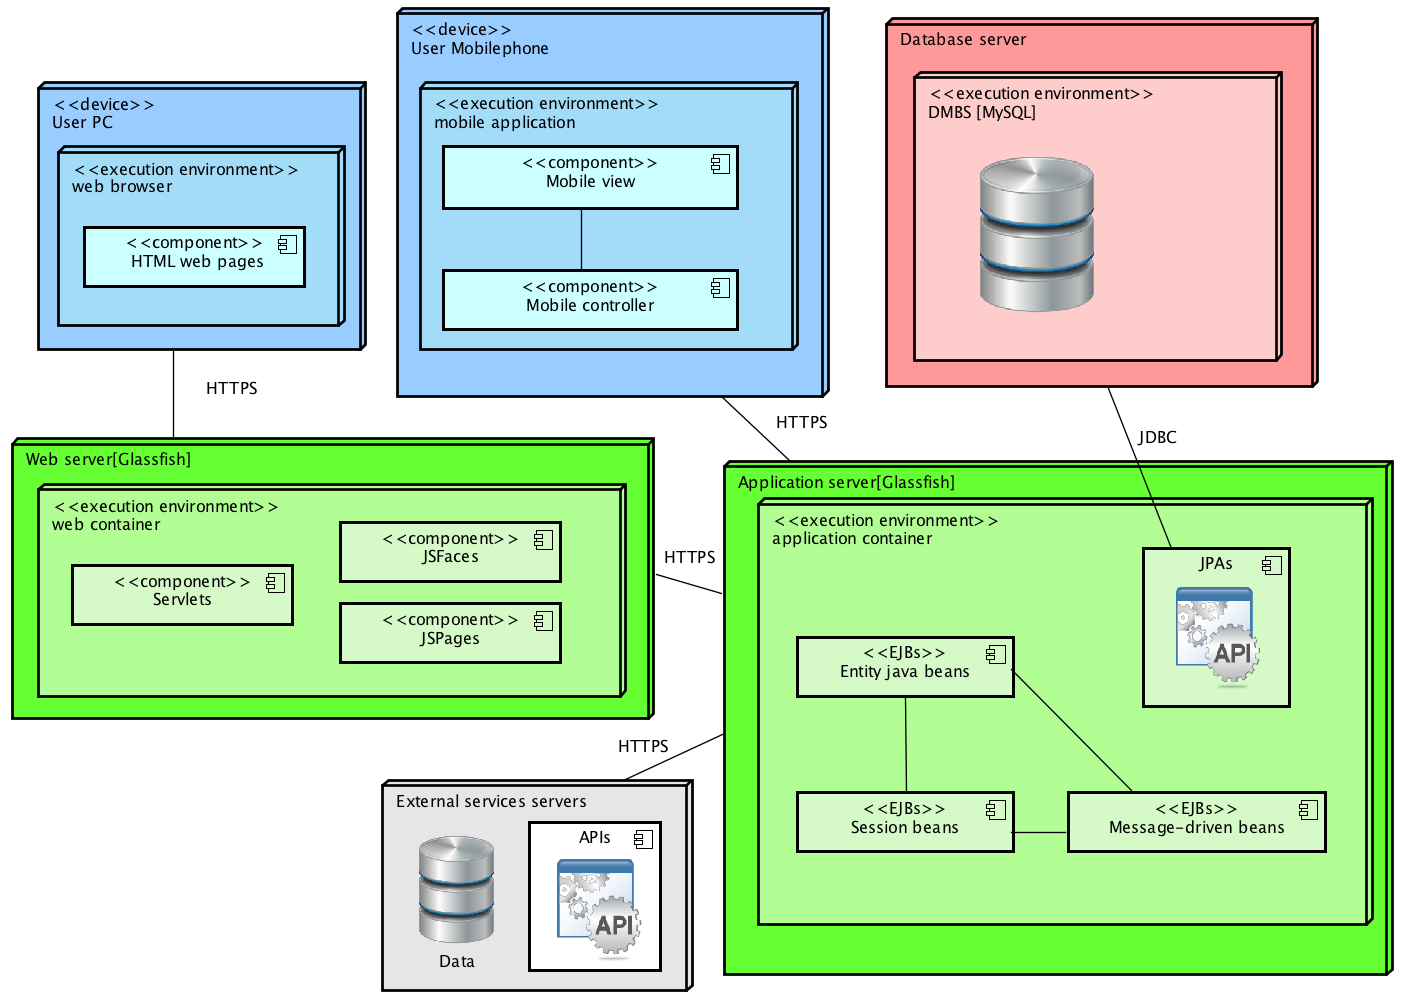
\includegraphics[width=1.5\linewidth]{images/deploymentdiagram} 
}
\caption{Deployment diagram} 
\label{fig:deploymentdiagram} 


\end{center}
\end{figure} 